\documentclass[border=1mm]{standalone}
%\documentclass[11pt]{article}
\usepackage{amsfonts,tikz,tikz-layers}
\usepackage{rotating}
\usetikzlibrary{fadings,quotes, shapes,calc,decorations.markings}
\usetikzlibrary{patterns}
\usetikzlibrary{shadows.blur}
\usetikzlibrary{shapes,shapes.geometric,positioning, arrows, arrows.meta}
\usetikzlibrary{backgrounds}

\begin{document}
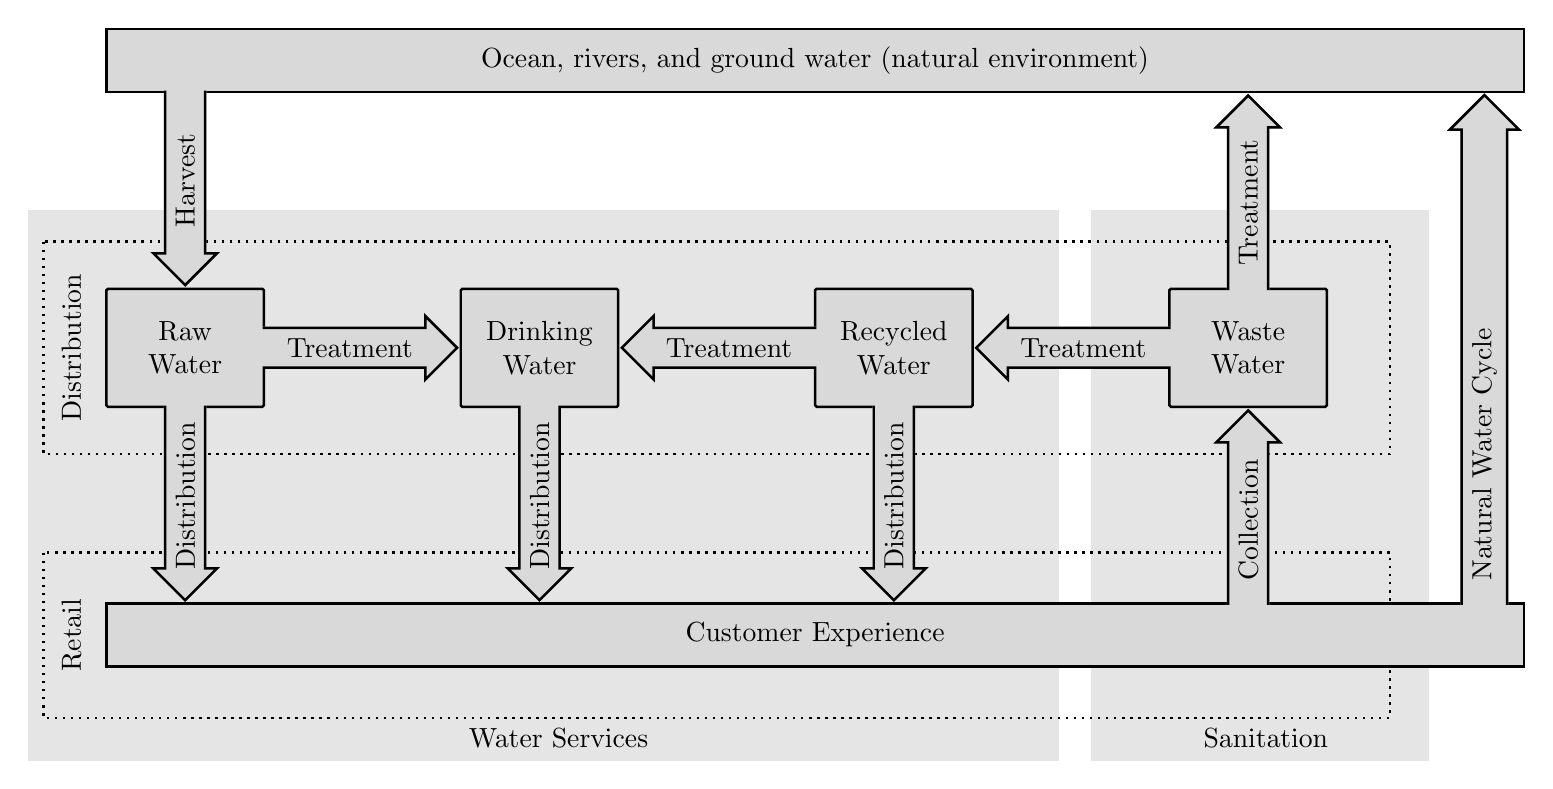
\begin{tikzpicture}[ line width=.9pt
  ]
% Arrow and block styles
\tikzstyle{arrow} = [draw=gray!30,fill=gray!30,anchor=west,outer sep=0pt,single arrow,draw, text width=1.95cm,align=center,single arrow head extend=.15cm,shape border rotate=0,text=black]
\tikzstyle{arrow2} = [draw=gray!30,fill=gray!30,anchor=east,outer sep=0pt,single arrow,draw, text width=1.95cm,align=center,single arrow head extend=.15cm,shape border rotate=180,text=black]
\tikzstyle{arrow3} = [draw=gray!30,fill=gray!30,anchor=north,outer sep=0pt,single arrow,draw, text height=1.95cm,align=center,single arrow head extend=.15cm, shape border rotate=270,text=black]
\tikzstyle{arrow4} = [draw=gray!30,fill=gray!30,anchor=south,outer sep=0pt,single arrow,draw, text height=1.95cm,align=center,single arrow head extend=.15cm, shape border rotate=90,text=black]
\tikzstyle{arrow5} = [draw=gray!30,fill=gray!30,anchor=south,outer sep=0pt,single arrow,draw, text height=5.92cm,align=center,single arrow head extend=.15cm, shape border rotate=90,text=black]

\tikzstyle{set}=[draw=black,fill=gray!30,outer sep=0pt, align=center, rounded corners=.2mm, minimum width=2cm, minimum height=1.5cm,text=black]
% Blocks
\node[set] (rw) {Raw\\Water};
\node[set, right=2.5cm of rw] (dw) {Drinking\\Water};
\node[set, right=2.5cm of dw] (rew) {Recycled\\Water};
\node[set, right=2.5cm of rew] (ww) {Waste\\Water};

\node[draw=black,fill=gray!30, minimum width=18cm,minimum height=.8cm, anchor=north west,text=black,outer sep=0pt] (cus) at ([yshift=-2.5cm]rw.south west) {Customer Experience};

\node[draw=black,,fill=gray!30, minimum width=18cm,minimum height=.8cm, anchor=south west,text=black,outer sep=0pt] (oc) at ([yshift=2.5cm]rw.north west) {Ocean, rivers, and ground water (natural environment)};

%\node[draw=black,,fill=gray!30, minimum width=6.5cm, minimum height=.8cm, anchor=south east,rotate=90,outer sep=0pt,text=black] at (oc.south east) {Natural Water Cycle};


% Horizontal arrows
\node [arrow,xshift=-.45pt] (ar1) at (rw.east) {Treatment};
\node [arrow2,xshift=.45pt] (ar2) at (rew.west) {Treatment};
\node [arrow2,xshift=.45pt] (ar3) at (ww.west) {Treatment};
% Vertical arrows
\coordinate (p1) at (cus.north);
\node [arrow3,yshift=.46pt] (ar4) at (rw.south) {\rotatebox{90}{Distribution}};
\node [arrow3,yshift=.46pt] (ar5) at (dw.south) {\rotatebox{90}{Distribution}};
\node [arrow3,yshift=.46pt] (ar6) at (rew.south) {\rotatebox{90}{Distribution}};
\node [arrow4,yshift=-.45pt] (ar7) at (p1-|ww.-90) {\rotatebox{90}{$\,\,\,$Collection}};
\coordinate (p2) at (oc.south);
\node [arrow3,yshift=.45pt] (ar8) at (p2-|rw) {\rotatebox{90}{$\quad$Harvest}};
\node [arrow4,yshift=-.45pt] (ar9) at (ww.90) {\rotatebox{90}{$\,\,\,$Treatment}};

\node[arrow5, yshift=-.45pt] (ar10) at ([yshift=-2.5cm, xshift=4cm]ww.south west) {\rotatebox{90}{$\,\,\,$Natural Water Cycle}};

\foreach \i in {1,...,10}
\draw[black, line width=.9pt] (ar\i.after tail)--(ar\i.before head)--(ar\i.before tip)--(ar\i.tip)--(ar\i.after tip)--(ar\i.after head)--(ar\i.before tail);
% Background rectangles
\begin{scope}[on behind layer]
\fill[gray!20] ([xshift=-1cm,yshift=1cm]rw.north west) rectangle ([xshift=1.1cm,yshift=-4.5cm]rew.south east);
\end{scope}

\begin{scope}[on behind layer]
\fill[gray!20] ([xshift=-1cm,yshift=1cm]ww.north west) rectangle ([xshift=1.3cm,yshift=-4.5cm]ww.south east);

\draw[black, dotted, line width=.9pt] ([xshift=-.8cm,yshift=.6cm]rw.north west) rectangle ([xshift=.8cm,yshift=-.6cm]ww.south east);
\node[rotate=90, anchor=south, text=black] at ([xshift=-.2cm]rw.west) {Distribution};

\begin{scope}[transform canvas={yshift=-3.65cm}]
\draw[black, dotted,line width=.9pt] ([xshift=-.8cm,yshift=.3cm]rw.north west) rectangle ([xshift=.8cm,yshift=-.3cm]ww.south east);
\node[rotate=90, anchor=south, text=black] at ([xshift=-.2cm]rw.west) {Retail};
\end{scope}
\end{scope}

\node[text=black] at ([yshift=-.9cm]cus.-173) {Water Services};
\node[text=black] at ([yshift=-.9cm]cus.-4) {Sanitation};
%---------------------
\end{tikzpicture}

\end{document}
